\chapter{Resultados e discussão}
\label{cap:resultados}

\begin{enumerate}
	
	\item Parágrafo de introdução do capítulo. Citar que, basicmente, o leitor encontrará no capítulo:
		\begin{enumerate}
			\item Resultados do ONEMAX, legitimando o uso do código para o programa mais complexo que foi utilizado no método dos indianos.
			\item o estudo dos tipos de \textit{fitness}, operador responsável pelo elo entre o algoritmo e o problema \cite{Linden2008}, que, para o nosso caso, é encontrar autovalores. Ponte para o próximo: para cada tipo de \textit{fitness}, um resultado diferente.
		\end{enumerate}

	\item Os dois tipos de fitness dos indianos. Ideia central: dois tipos, resultados diferentes. Com $\nabla \rho$ chegamos a um autovalor qualquer, com $(\rho - \rho_0)^2$ podemos chegar ao mínimo, mas dá mais trabalho. Ponte para o próximo: proposta de dois novos fitness.
	
	\item Combinação de $\nabla \rho$ com $(\rho - \rho_0)^2$. Se cada forma leva a comportamentos diferentes, tentamos combinar os dois termos em um único fitness. Uma hipótese seria a melhoria da qualidade dos resultados. A hipótese não foi confirmada. Ponte para o próximo: a busca pela qualidade levou à verificação da importância do parâmetro $\lambda$.
	
	\item Além do que os indianos disseram, que $\lambda$ é escolhido para não estourar a função exponencial, ele tem influência na convergência do algoritmo e na precisão (ou resolução) do fitness. Se na primeira população, geração inicial, o fitness médio é alto, isso provoca convergência precoce, fazendo com que o resultado final seja ruim. Por outro lado, se no início o fitness médio é muito baixo, não há muita discriminação entre os indivíduos, o fitness não cresce e não chegamos a uma solução. A medida que o fitness se aproxima de 1, a discriminação entre os indivíduos fica difícil, levando ao problema da resolução. Ponte para o próximo: vários testes levaram ao desenvolvimento de uma equação empírica para $\lambda$, restrita às matrizes de Coope$-$Sabo \cite{Coope1977}.
	
	\item Fórmula empírica. Por já conhecermos de antemão os autovalores das matrizes de Coope$-$Sabo, foi possível criar uma fórmula empírica para $\lambda$. Ela garante que na primeira população o \textsl{fitness} médio é baixo, previnindo o \textsl{underflow} do \textit{fitness} e a convergência prematura.
	
	\end{enumerate}
	
\section{O método não leva ao mínimo global}	
	
	Na seção \ref{sec:metodo} vimos no artigo \cite{metodo2004} que o \textit{fitness} utilizado foi
	
	\begin{equation}
		\label{eq:fitnessGrad2}
		f_i = e^{-\lambda \| \nabla \rho_i \|^2},
	\end{equation}
	onde $f_i$ é o \textit{fitness} do $i$-ésimo indivíduo da população, $\lambda$ é um parâmetro para evitar o estouro do \textit{fitness} e $\| \nabla \rho_i\|^2$ é o módulo ao quadrado do vetor gradiente de $\rho$, dado por
		
				\begin{equation}
					\nabla \rho_i = \frac{2[H - \rho_i]C_i}{C_i^t C_i},
				\end{equation}
	em que $C_i$ é um vetor candidato à solução do problema do autovalor
	
	\begin{equation}
		HC = EC.
	\end{equation}
	
	A fim de reproduzir os resultados, testamos o método com matrizes de Coope\-Sabo de ordem 10, 20, 30 e 40, utilizando os mesmos parâmetros encontrados em \cite{metodo2004}: probabilidade de \textit{crossover} $p_c = 75\%$, probabilidade de mutação $p_m = 50\%$ e intensidade de mutação $\Delta = 0,01$. Com um bom ajuste de $\lambda$, que será discutido em detalhes posteriormente, o \textit{fitness} comportou-se conforme o esperado em todos os casos. Um exemplo está na figura \ref{fig:compFitnessTipo1N10}, que apresenta o melhor fitness de cada geração para uma matriz de ordem N = 10. Na primeira geração o melhor \textit{fitness} é pequeno, aproximadamente 0,1, cresce rapidamente e a partir da décima geração está próximo de 1.
	
	\begin{figure}[htbp]
		\centering
			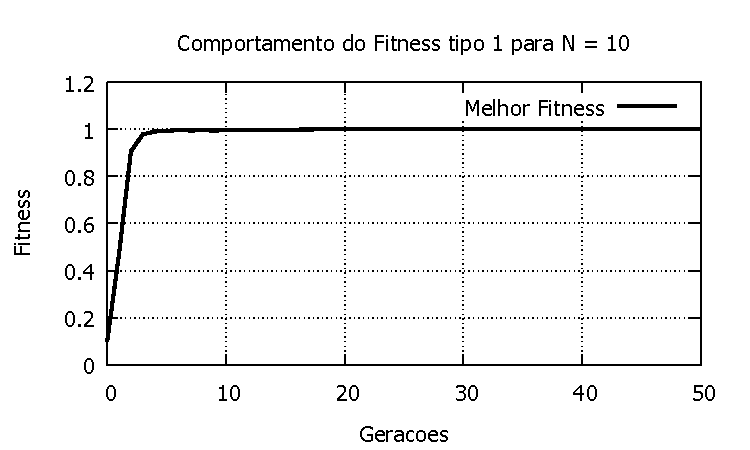
\includegraphics{figs/resultados/compFitnessTipo1N10.pdf}
			\caption{Comportamento do \textsl{fitness} tipo 1 para N = 10. Na primeira geração o melhor \textit{fitness} é pequeno, aproximadamente 0,1, cresce rapidamente e a partir da décima geração está próximo de 1.}
		\label{fig:compFitnessTipo1N10}
	\end{figure}
	
	O próximo passo foi verificar o comportamento de $\rho$, o Quociente de Rayleigh, e, especificamente, sua convergência para o menor autovalor $E_0$. Ainda conforme \cite{metodo2004}, obteríamos uma curva semelhante à da figura \ref{fig:compFitnessTipo1N10}, mas invertida, ou seja, os primeiros valores de $\rho$ seriam grandes e, rapidamente, diminuiriam até haver convergência para o autovalor mínimo. Na figura \ref{fig:rho_N10} há um exemplo.	Os gráficos exibem os valores de $\rho$ para a mesma execução apresentada na figura \ref{fig:compFitnessTipo1N10}. Note no primeiro gráfico que até a geração 20 o quociente $\rho$ teve caráter oscilatório e, então, aparentemente estabilizou-se entre 6 e 8, valores muito superiores ao autovalor mínimo para essa matriz, $E_0 = 0,38675$. Entretanto, ainda no primeiro gráfico, observa-se que há uma tendência de queda do $\rho$ entre as gerações 40 e 50 e, portanto, existiria a possibilidade do algoritmo convergir para $E_0$. Porém, para esse exemplo especificamente, isso não aconteceu, como pode ser visto no segundo gráfico da figura \ref{fig:rho_N10}. Para garantir a estabilidade, o programa foi executado até a geração 400.000, e o valor médio obtido foi $<\rho> = 6,572898$. Para nossa surpresa, além do valor obtido de $\rho$ para o melhor indivíduo não ser o mínimo, ele não é um valor qualquer, mas corresponde, com erro menor que $0,00002\%$, ao quarto autovalor da matriz, $E_3 = 6,572897$. Um gráfico expandido dessa execução está na figura \ref{fig:rho_N10_completa} da página \pageref{fig:rho_N10_completa}. Pensamos, então, que poderia haver algo de errado com o nosso programa. 
	
	\begin{figure}[htbp]
		\centering
			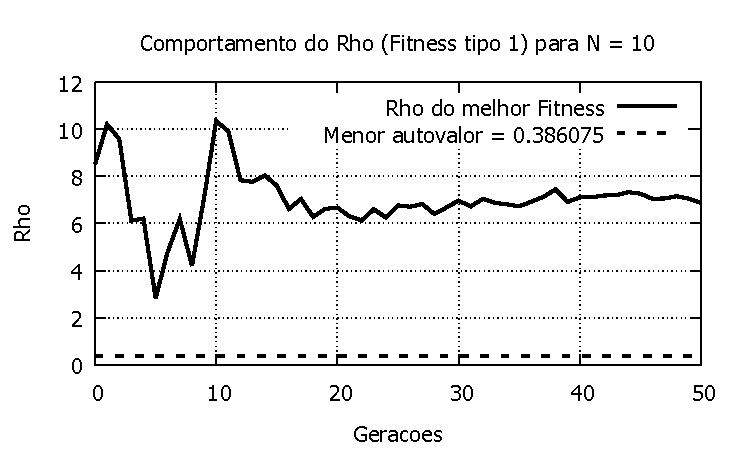
\includegraphics[width=0.40\textwidth]{figs/resultados/rho_N10_g50.pdf}
			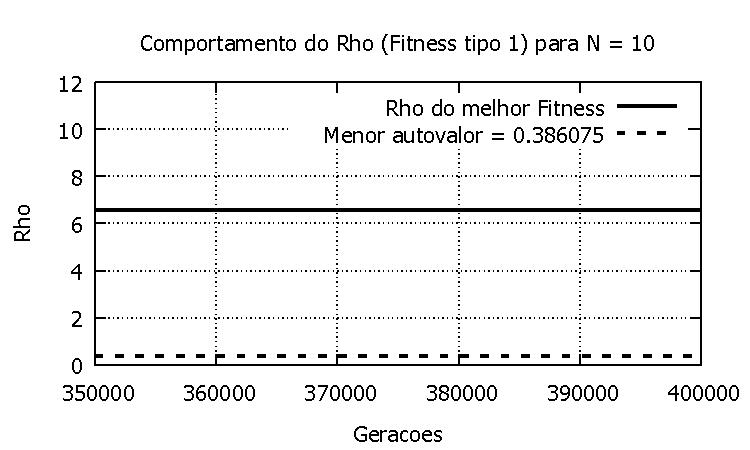
\includegraphics[width=0.40\textwidth]{figs/resultados/rho_N10_g400000.pdf}
		\caption{Comportamento de $\rho$ (Quociente de Rayleigh) para uma matriz de Coope$-$Sabo de ordem 10.}
		\label{fig:rho_N10}
	\end{figure}
	
	\newpage
	\begin{landscape}
	\begin{figure}[p]
		\centering
			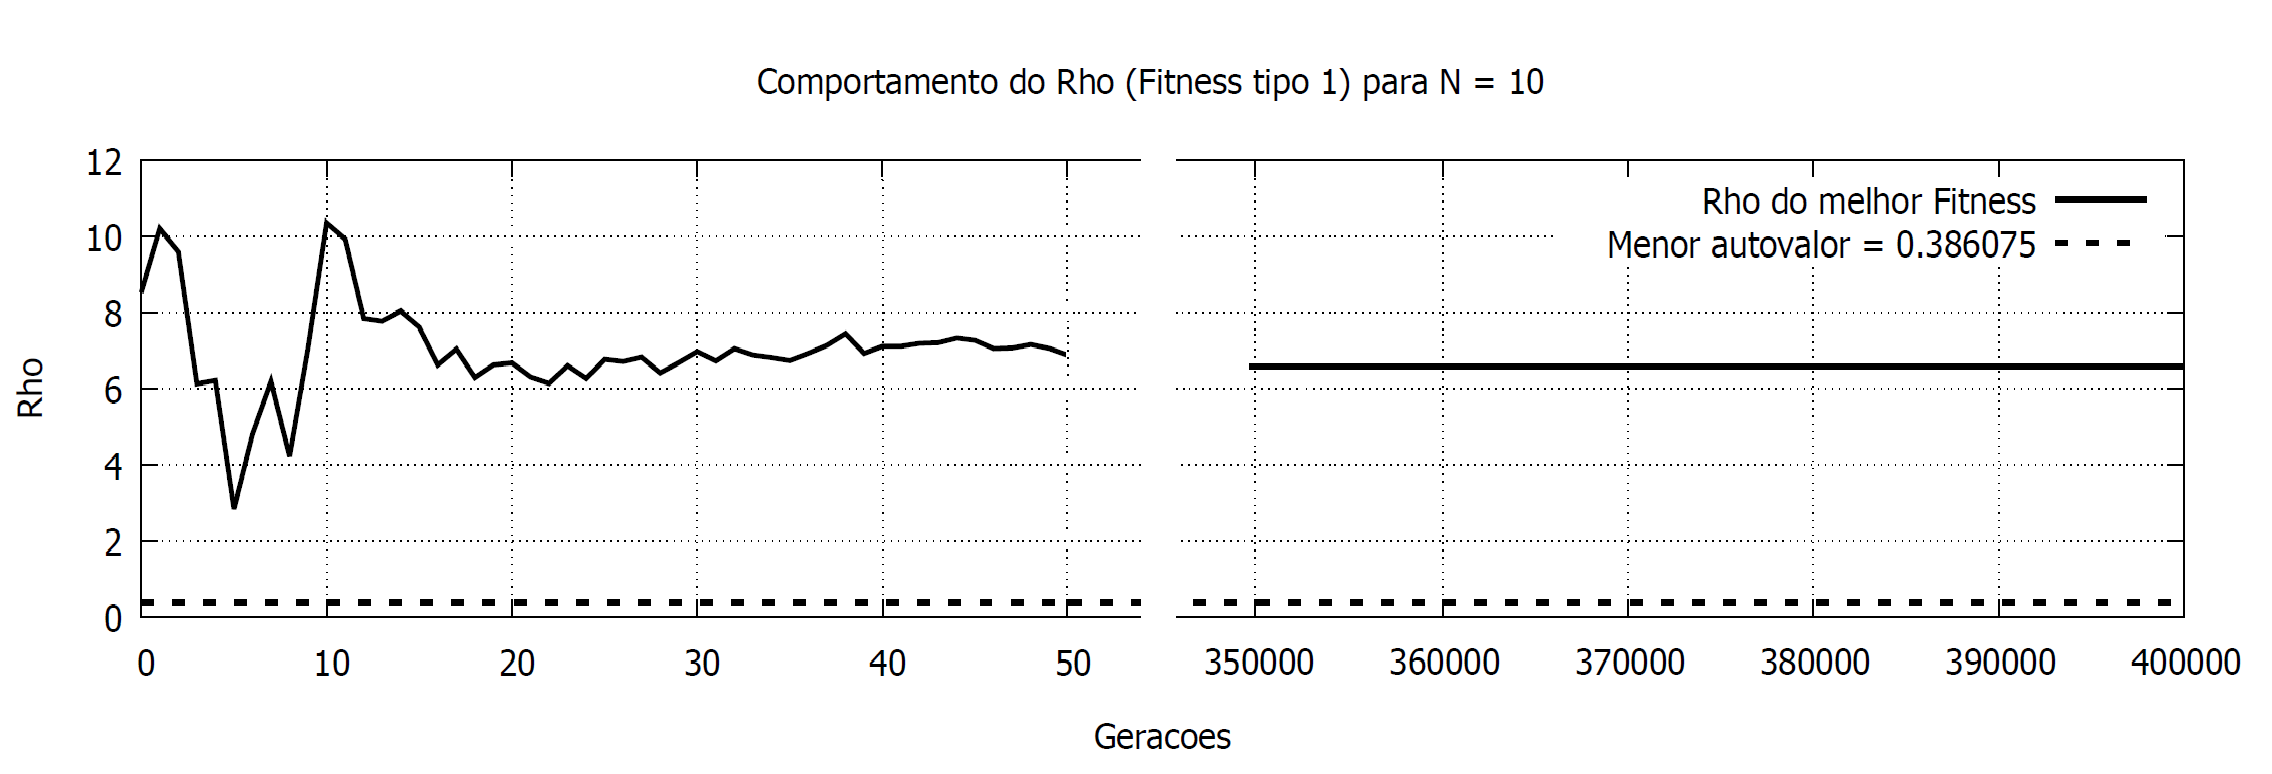
\includegraphics[width=1.3\textwidth]{figs/resultados/rho_N10.png}
		\caption{Comportamento de $\rho$ (Quociente de Rayleigh) para uma matriz de Coope$-$Sabo de ordem 10.}
		\label{fig:rho_N10_completa}
	\end{figure}
	\end{landscape}
	\newpage
			
	Após esses resultados preliminares executamos uma validação cuidadosa do programa, testando cada uma de suas quase 2500 linhas e comparando os resultados das operações e cálculos com os softwares Excel \cite{excel} e SciLab \cite{scilab}. A hipótese era a de que erros numéricos, principalmente nas funções de álgebra linear e nos operadores genéticos, pudessem ter levado ao comportamento incorreto da não convergência para o menor autovalor. De fato alguns erros foram encontrados.
	
	Discutiremos a seguir os testes com a versão corrigida do programa e exibidos nas figuras \ref{fig:execucoes_N10}, \ref{fig:execucoes_N20}, \ref{fig:execucoes_N30} e \ref{fig:execucoes_N40}. Visando brevidade, apresentaremos dados para matrizes de Coope\-Sabo de ordem 10, 20, 30 e 40, sem perda de generalidade. Foram cinco execuções para cada matriz, até a geração 400.000, gerando sempre dois gráficos, um do comportamento do \textit{fitness} médio (<\textit{fitness}>) e outro do comportamento do Quociente de Rayleigh médio (<$\rho$>), ambos em função do número de gerações, e dando ênfase às primeiras 100 gerações. Essas escolhas, número máximo da geração e uso de médias sobre cada população, visaram garantir, respectivamente, a convergência genética e boa precisão. A exibição de apenas as primeiras 100 gerações tem como objetivo olhar em detalhe (com \textit{zoom}) o momento em que o \textit{crossover} tem mais peso, ou seja, onde há geralmente os saltos no espaço de soluções de um Algoritmo Genético. Em todos os gráficos de $<\rho>$ há indicado nas legendas o autovalor mínimo $E_0$ e o autovalor obtido após as 400.000 gerações ($E_{obtido}$). Na tabela \ref{tab:autovalores10a40} há a lista de todos os autovalores. Por exemplo, para uma matriz de ordem $N = 10$, o menor autovalor é $E_0 = $0,386075, e o quinto autovalor para $N = 30$ é $E_4$ = 8,450274.
	
	Comecemos a discussão com o que foi encontrado em todas as execuções. Em qualquer gráfico do \textit{fitness} observa-se estabilidade do comportamento conforme esperado pelo método: no início seu valor é baixo, próximo de zero, cresce rapidamente nas primeiras gerações e fica estável próximo de $<fitness> = 1$. Com relação ao $\rho$, há sempre oscilações, sejam pequenas variações em torno de uma clara linha de tendência, como nas execuções 02 para N = 10, ou grandes saltos, como na execução 05 de N = 20 e 05 de N = 30. Novamente, o menor autovalor não foi obtido em nenhuma execução, contradizendo os resultados de \cite{metodo2004}, mas, por outro lado, o algoritmo sempre encontrou algum autovalor.

\newpage	
\begin{figure}[phtb]
\centering
  \begin{tabular}{@{}cc@{}}
    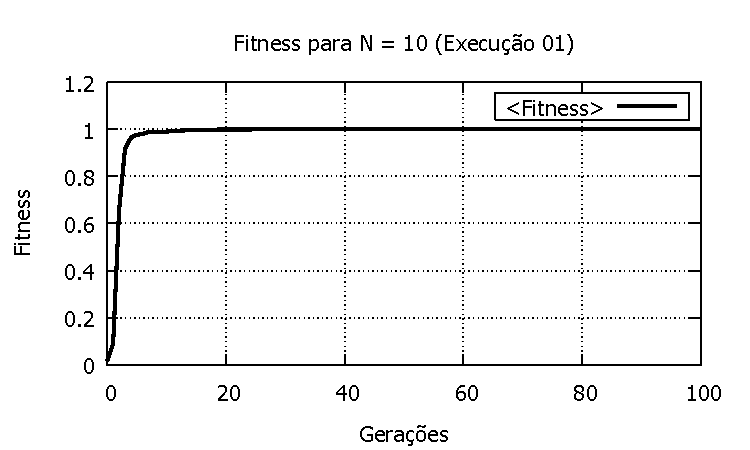
\includegraphics[width=.40\textwidth]{figs/resultados/N10_01_fitness.pdf} &
    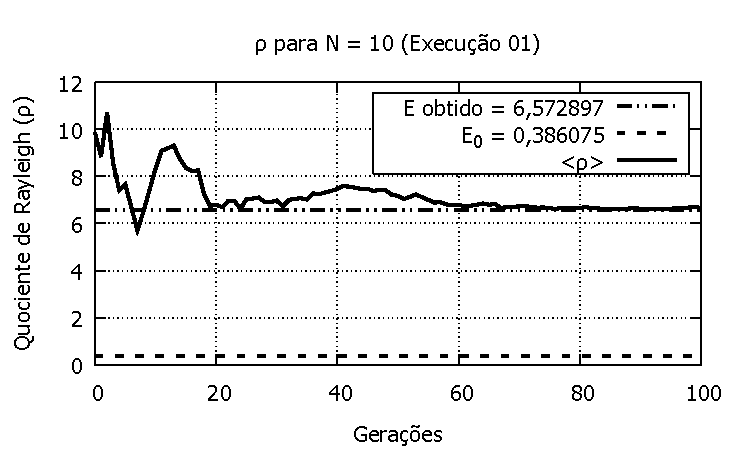
\includegraphics[width=.40\textwidth]{figs/resultados/N10_01_rho.pdf}   \\
		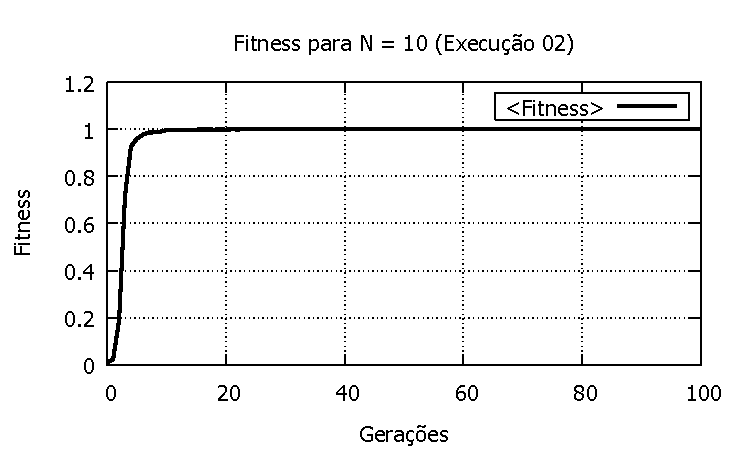
\includegraphics[width=.40\textwidth]{figs/resultados/N10_02_fitness.pdf} &
    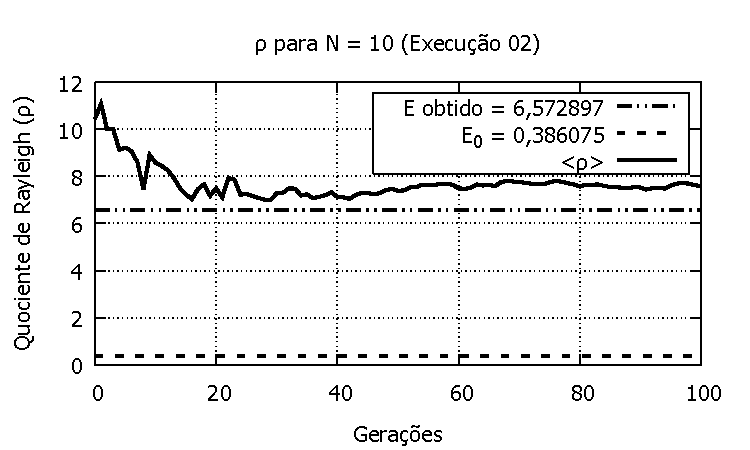
\includegraphics[width=.40\textwidth]{figs/resultados/N10_02_rho.pdf}   \\
		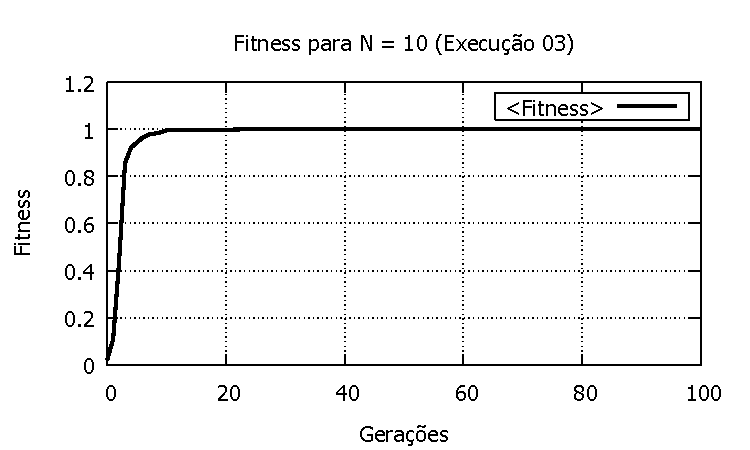
\includegraphics[width=.40\textwidth]{figs/resultados/N10_03_fitness.pdf} &
    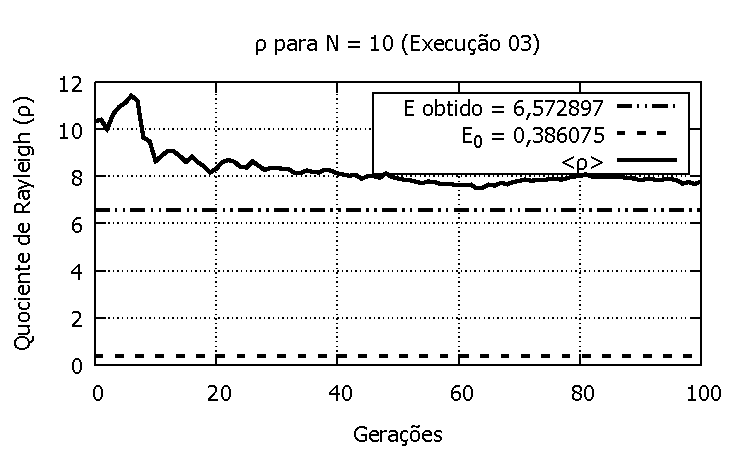
\includegraphics[width=.40\textwidth]{figs/resultados/N10_03_rho.pdf}   \\
		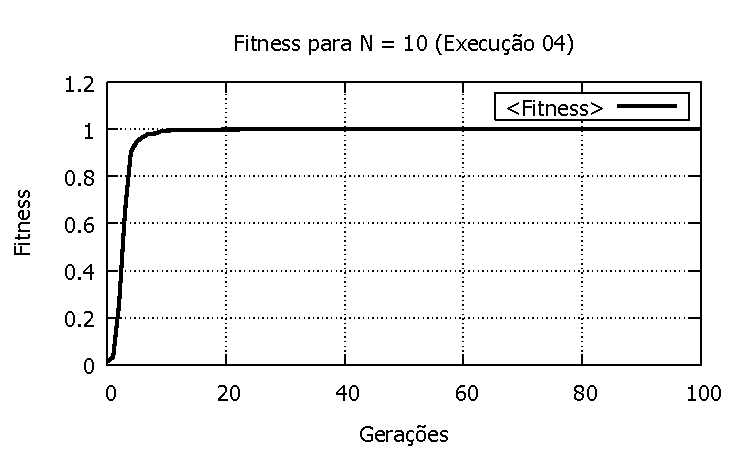
\includegraphics[width=.40\textwidth]{figs/resultados/N10_04_fitness.pdf} &
    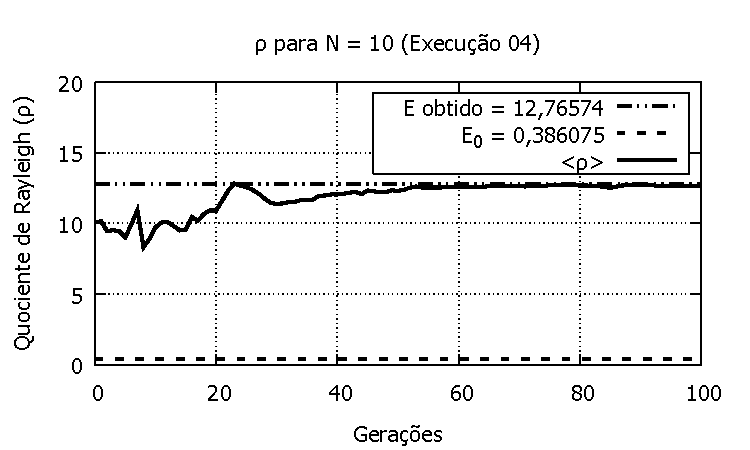
\includegraphics[width=.40\textwidth]{figs/resultados/N10_04_rho.pdf}   \\
		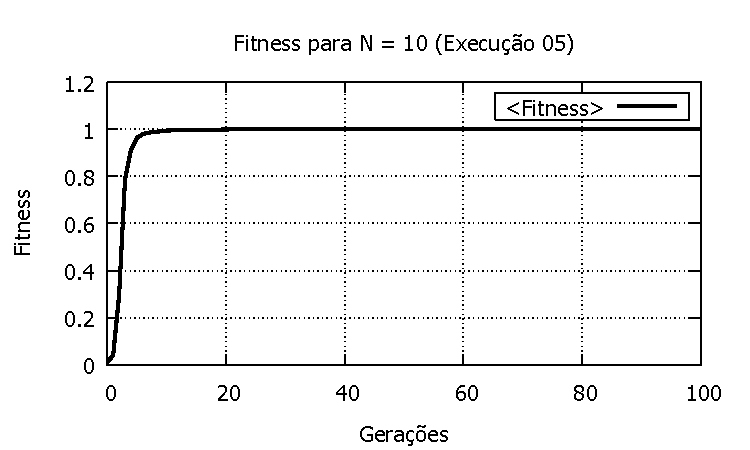
\includegraphics[width=.40\textwidth]{figs/resultados/N10_05_fitness.pdf} &
    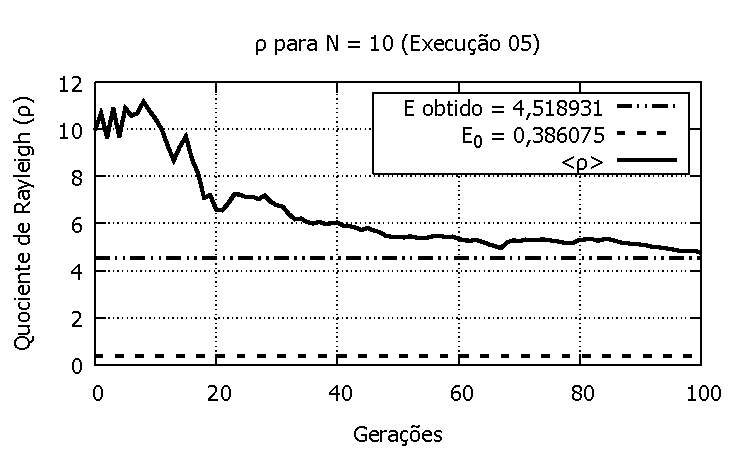
\includegraphics[width=.40\textwidth]{figs/resultados/N10_05_rho.pdf}
    %\multicolumn{2}{c}{\includegraphics[width=.23\textwidth]{example-image-a}}
  \end{tabular}
  \caption{Execuções N = 10.}
	\label{fig:execucoes_N10}
\end{figure}
\newpage
	
De fato, verificando os dados da tabela \ref{tab:execucoes10a40}, concluímos que tais valores não devem ser coincidência. Para todas as execuções o \textit{fitness} médio chegou ao valor máximo ($<f> = 1,000000$). As médias de $\rho$ sobre todos os indivíduos da última população possuem baixo desvio padrão ($\sigma$ < 0,0001), indicando que eles são muito parecidos e que o algoritmo atingiu a convergência genética. Ou seja, não há mais na população variabilidade genética suficiente para alterar o rumo da busca de modo a atingir o menor autovalor, ou o mínimo global. Portanto, o algoritmo chegou em um mínimo local, corroborado pelos baixos erros relativos de $<\rho>$ quando comparado com o autovalor mais próximo. Por exemplo, para N = 30, execução 4,  $<\rho>$ = 40,772447, correspondendo, com erro relativo menor que $-0,001\%$, ao vigésimo primeiro autovalor, $E_{20} = 40,772850$. Apesar das evidências descritas acima, até esse ponto ainda há dúvidas sobre a validade do nosso programa e, obviamente, dos resultados que dele saíram. Então, buscamos embasamento mais rigoroso.

De acordo com \cite{metodo2004}, se algum $C_i$, em algum momento, é o autovetor fundamental (associado ao menor autovalor), o $\nabla \rho$ é nulo. Com o \textit{fitness} da equação \eqref{eq:fitnessGrad2} os autores afirmam\footnote{Tradução livre de ``\textit{Clearly, $f_i \rightarrow 1$, as $\nabla \rho_i \rightarrow 0$, signalling that the evolution has hit the true ground state eigenvector of $H$ in the vector $C_i$}''.} que ``\textit{Claramente, $f_i \rightarrow 1$ quando $\nabla \rho_i \rightarrow 0$, sinalizando que a evolução atingiu o verdadeiro autovetor fundamental de $H$ em $C_i$}''. Há duas relações distintas de causalidade nessa frase, e acreditamos que nelas residam a explicação dos resultados obtidos por nós até agora.

A primeira relação de causalidade refere-se à afirmação ``\textit{$f_i \rightarrow 1$ quando $\nabla \rho_i \rightarrow 0$}'', que está absolutamente correta. Retomando a seção \ref{cap:metodo}, o \textit{fitness} definido pela equação \ref{eq:fitnessGrad2} é limitado no intervalo (0,1] e, como $\lambda > 0$, só chega ao seu valor máximo quando $\nabla \rho_i = 0$. Em outras palavras, $\nabla \rho_i \rightarrow 0$ implica $f_i \rightarrow 1$.

Na afirmação ``(...) sinalizando que a evolução atingiu o verdadeiro autovetor fundamental de $H$ em $C_i$}'' reside a segunda relação de causalidade que, apesar de sutil, é muito poderosa: se $f_i \rightarrow 1$, $C_i = C_0$.
	
\begin{figure}[phtb]
\centering
  \begin{tabular}{@{}cc@{}}
    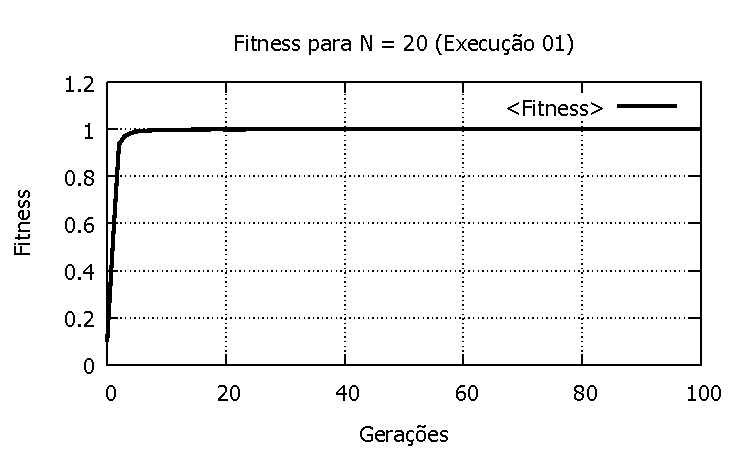
\includegraphics[width=.40\textwidth]{figs/resultados/N20_01_fitness.pdf} &
    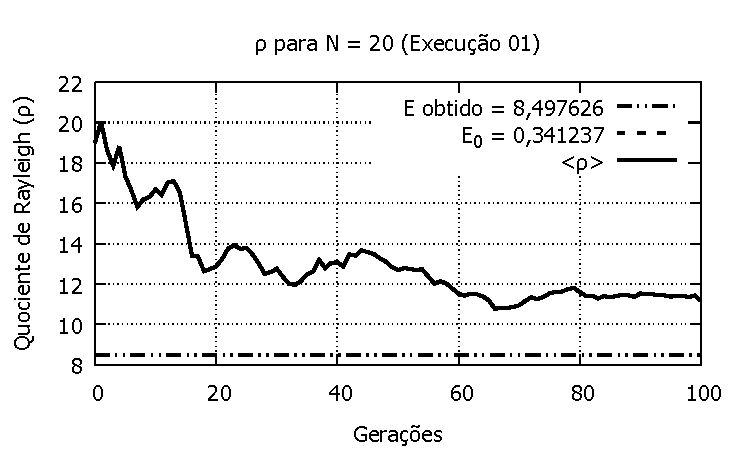
\includegraphics[width=.40\textwidth]{figs/resultados/N20_01_rho.pdf}   \\
		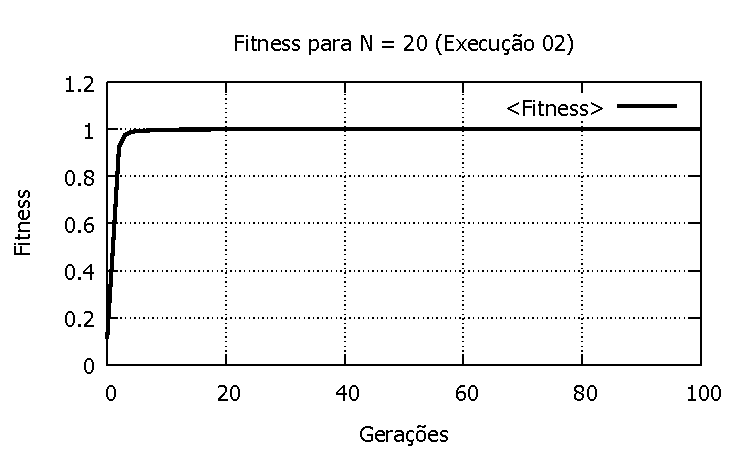
\includegraphics[width=.40\textwidth]{figs/resultados/N20_02_fitness.pdf} &
    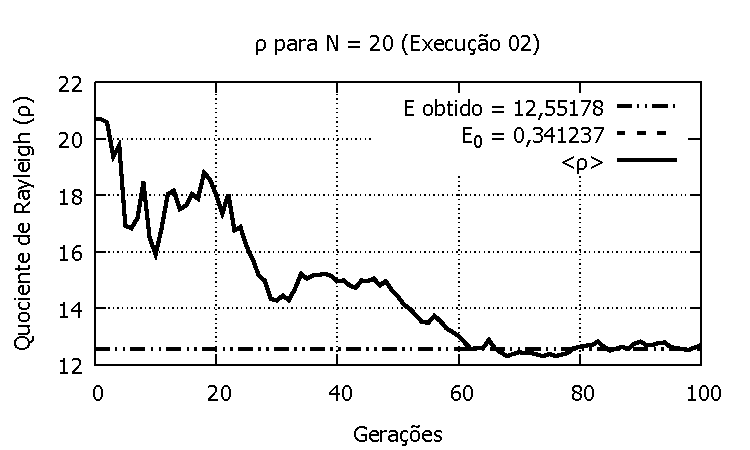
\includegraphics[width=.40\textwidth]{figs/resultados/N20_02_rho.pdf}   \\
		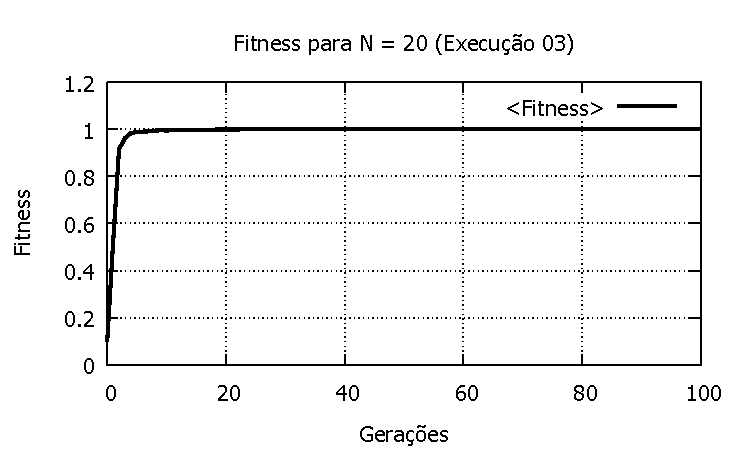
\includegraphics[width=.40\textwidth]{figs/resultados/N20_03_fitness.pdf} &
    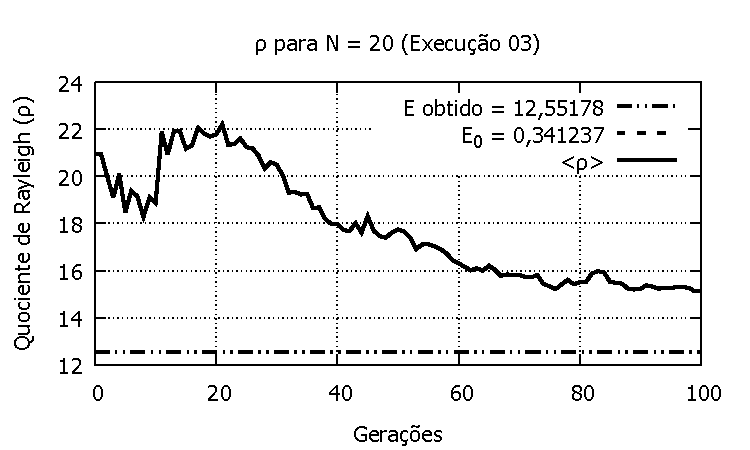
\includegraphics[width=.40\textwidth]{figs/resultados/N20_03_rho.pdf}   \\
		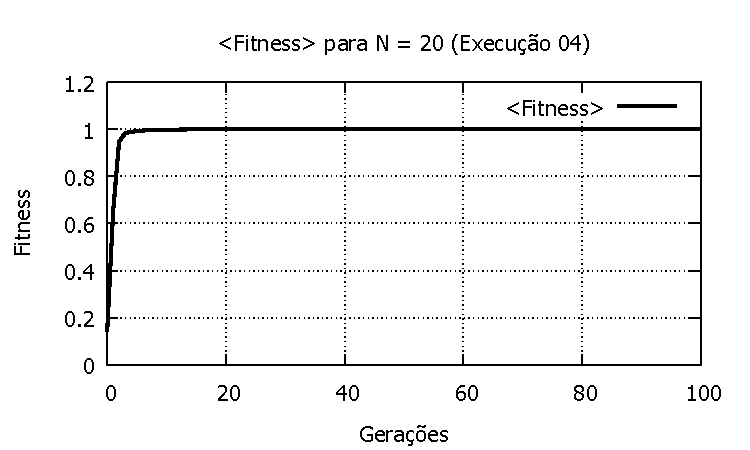
\includegraphics[width=.40\textwidth]{figs/resultados/N20_04_fitness.pdf} &
    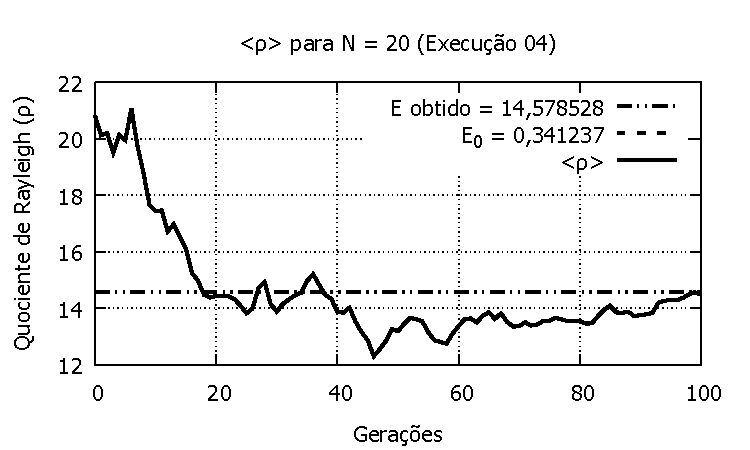
\includegraphics[width=.40\textwidth]{figs/resultados/N20_04_rho.pdf}   \\
		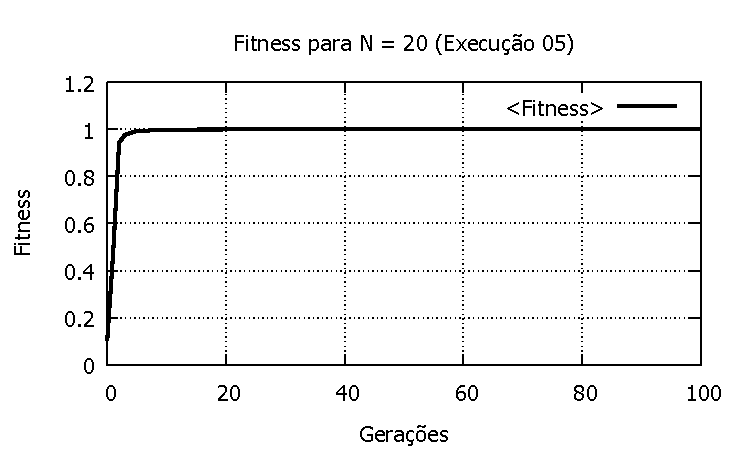
\includegraphics[width=.40\textwidth]{figs/resultados/N20_05_fitness.pdf} &
    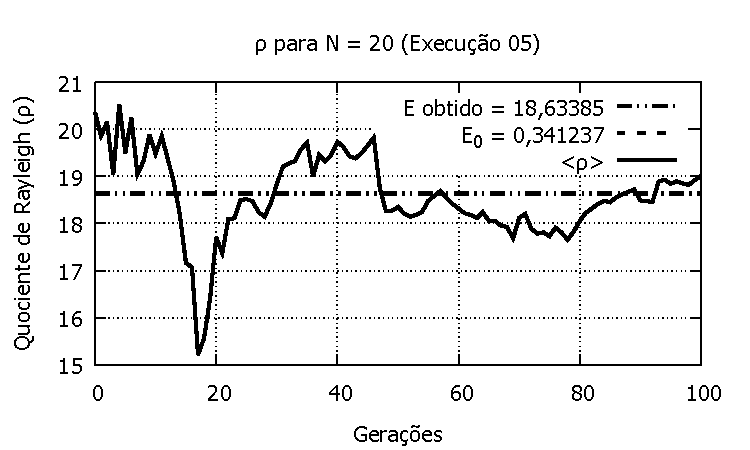
\includegraphics[width=.40\textwidth]{figs/resultados/N20_05_rho.pdf}
    %\multicolumn{2}{c}{\includegraphics[width=.23\textwidth]{example-image-a}}
  \end{tabular}
  \caption{Execuções N = 20.}
	\label{fig:execucoes_N20}
\end{figure}

\begin{figure}[phtb]
\centering
  \begin{tabular}{@{}cc@{}}
    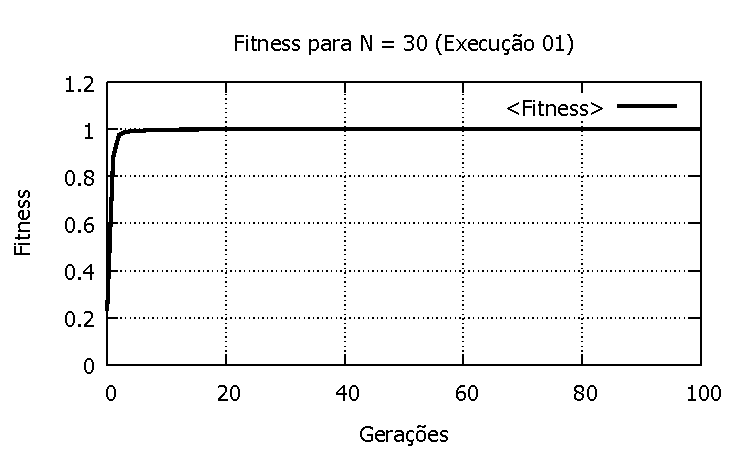
\includegraphics[width=.40\textwidth]{figs/resultados/N30_01_fitness.pdf} &
    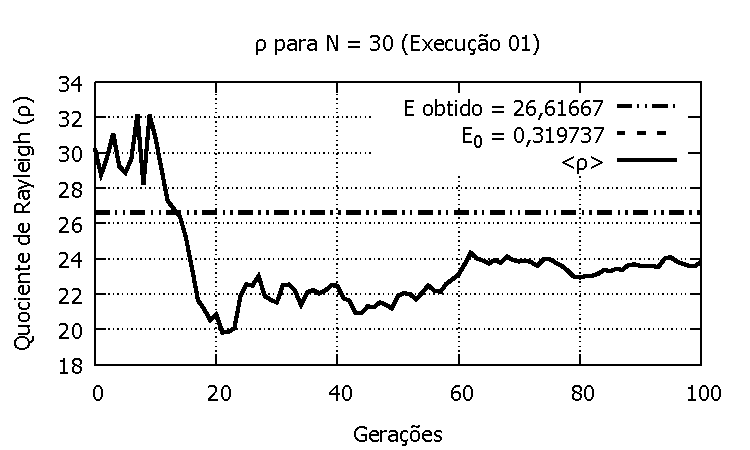
\includegraphics[width=.40\textwidth]{figs/resultados/N30_01_rho.pdf}   \\
		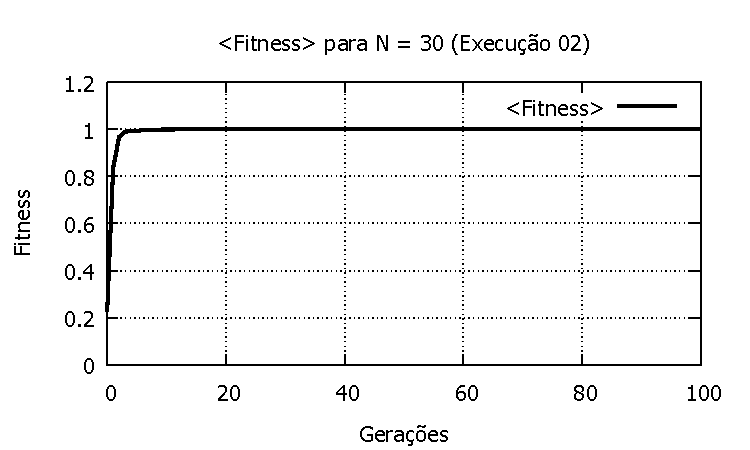
\includegraphics[width=.40\textwidth]{figs/resultados/N30_02_fitness.pdf} &
    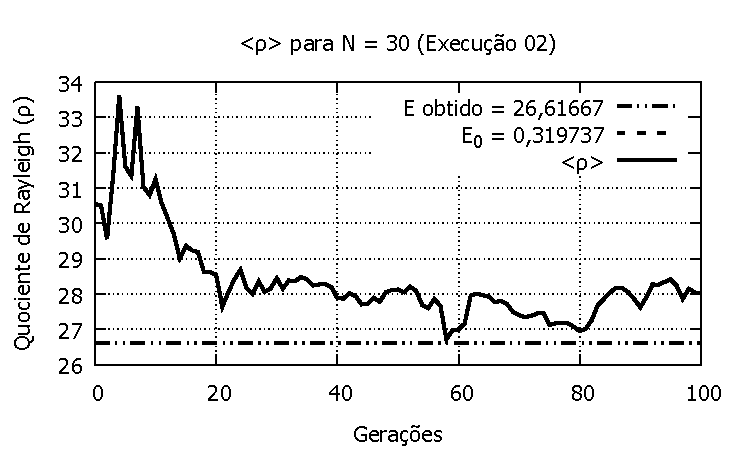
\includegraphics[width=.40\textwidth]{figs/resultados/N30_02_rho.pdf}   \\
		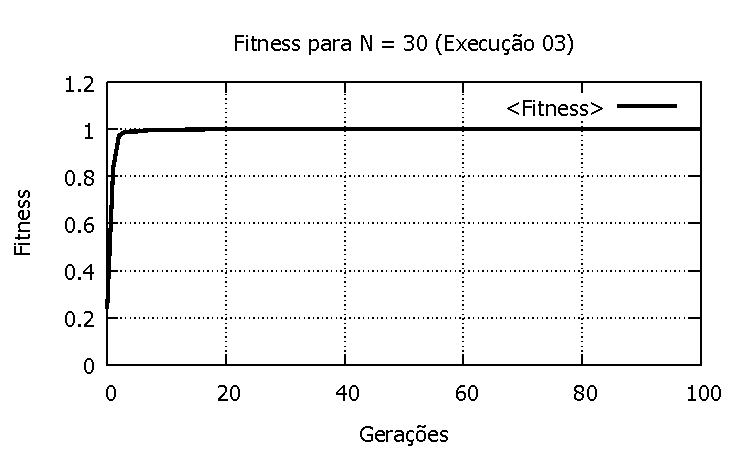
\includegraphics[width=.40\textwidth]{figs/resultados/N30_03_fitness.pdf} &
    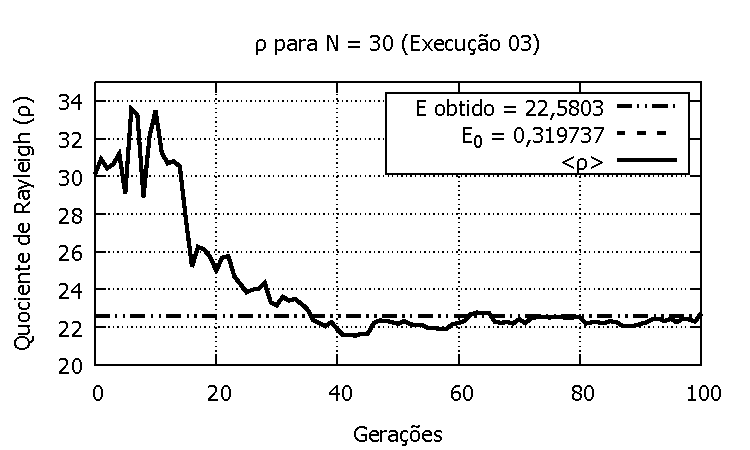
\includegraphics[width=.40\textwidth]{figs/resultados/N30_03_rho.pdf}   \\
		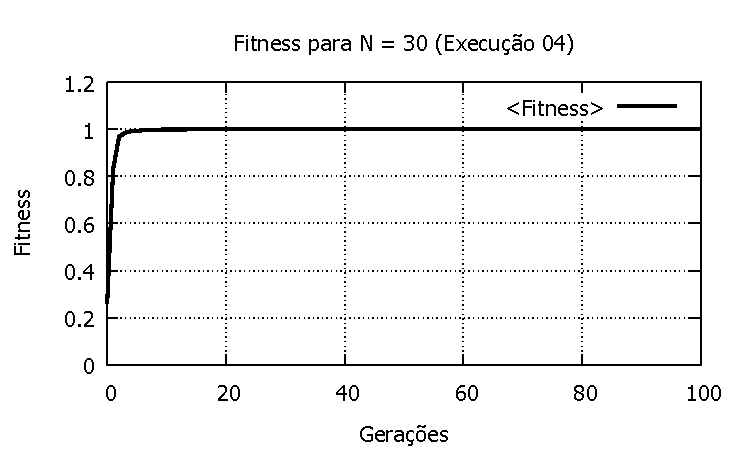
\includegraphics[width=.40\textwidth]{figs/resultados/N30_04_fitness.pdf} &
    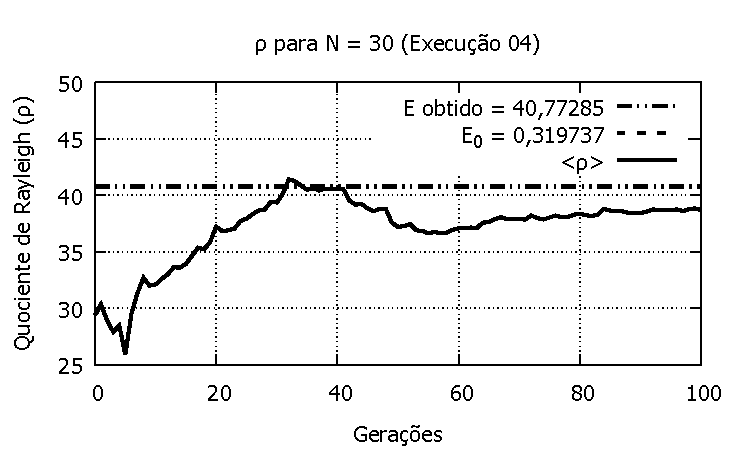
\includegraphics[width=.40\textwidth]{figs/resultados/N30_04_rho.pdf}   \\
		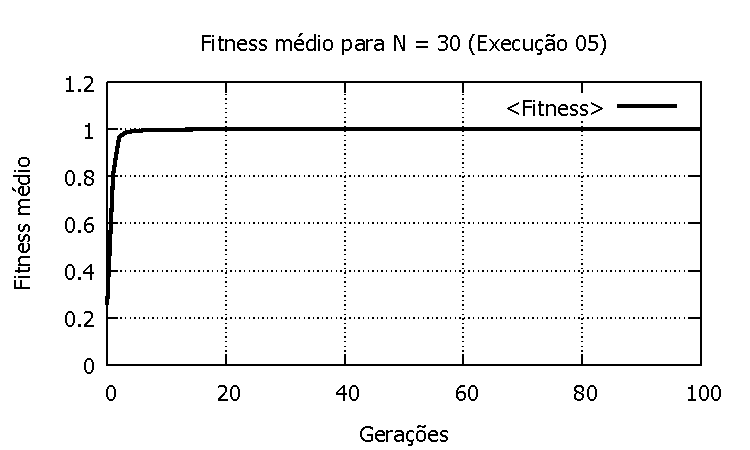
\includegraphics[width=.40\textwidth]{figs/resultados/N30_05_fitness.pdf} &
    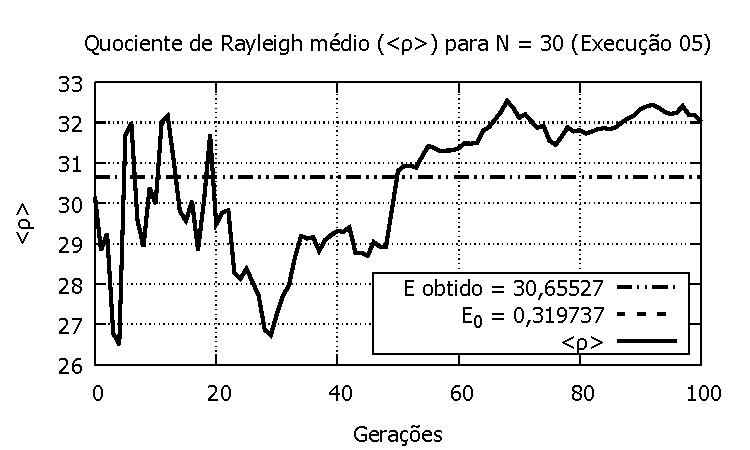
\includegraphics[width=.40\textwidth]{figs/resultados/N30_05_rho.pdf}
    %\multicolumn{2}{c}{\includegraphics[width=.23\textwidth]{example-image-a}}
  \end{tabular}
  \caption{Execuções N = 30.}
	\label{fig:execucoes_N30}
\end{figure}

\begin{figure}[phtb]
\centering
  \begin{tabular}{@{}cc@{}}
    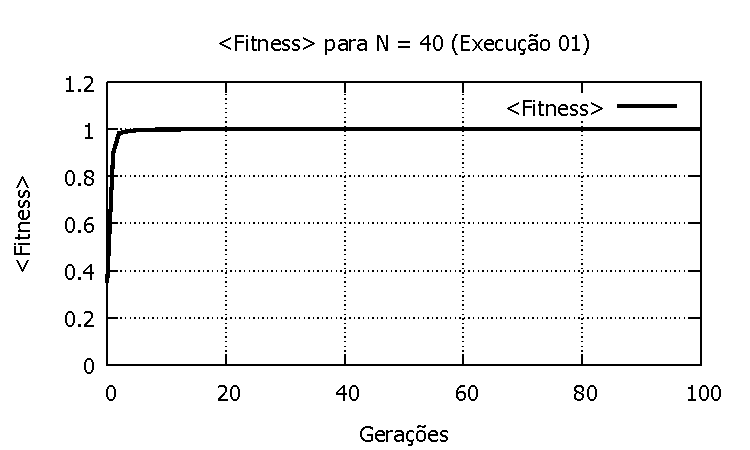
\includegraphics[width=.40\textwidth]{figs/resultados/N40_01_fitness.pdf} &
    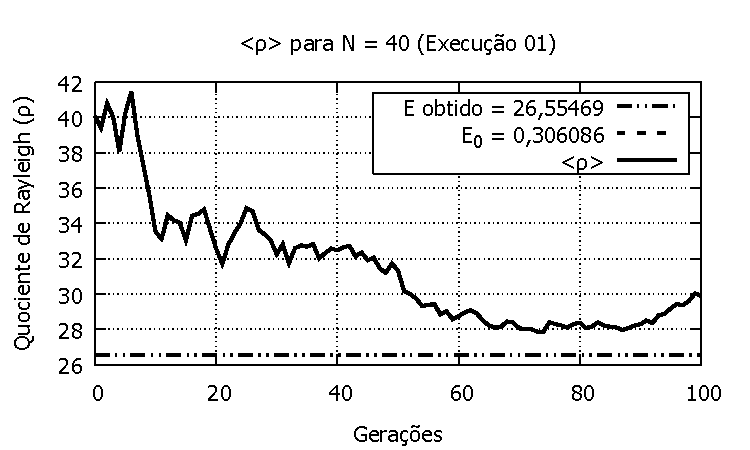
\includegraphics[width=.40\textwidth]{figs/resultados/N40_01_rho.pdf}   \\
		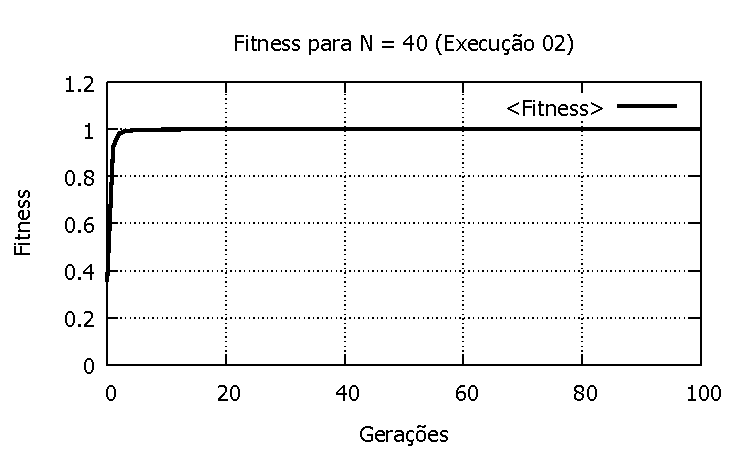
\includegraphics[width=.40\textwidth]{figs/resultados/N40_02_fitness.pdf} &
    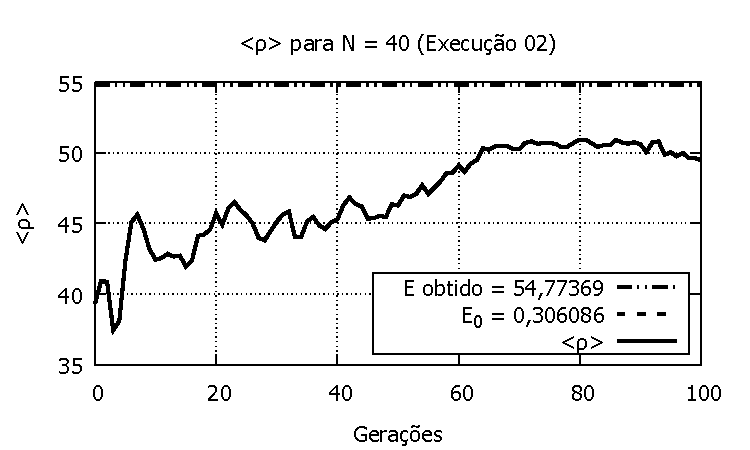
\includegraphics[width=.40\textwidth]{figs/resultados/N40_02_rho.pdf}   \\
		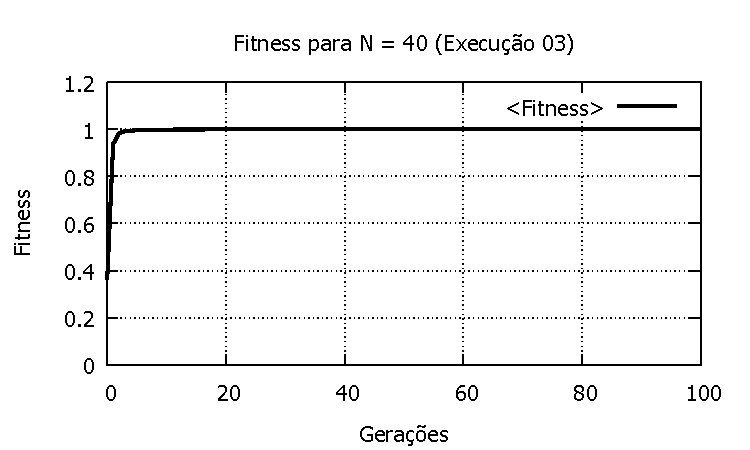
\includegraphics[width=.40\textwidth]{figs/resultados/N40_03_fitness.pdf} &
    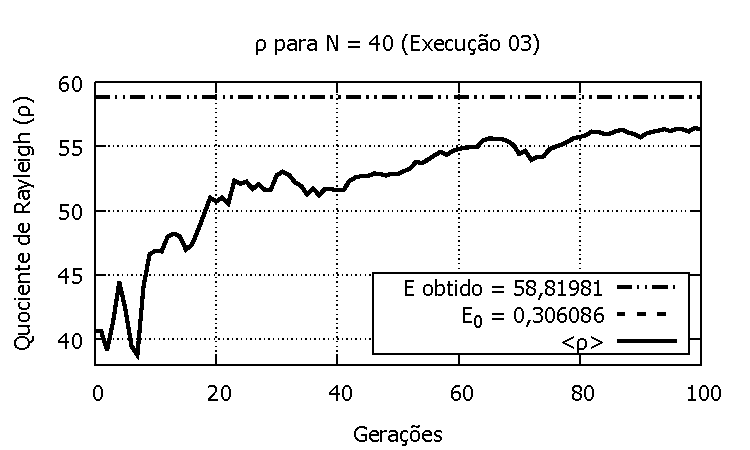
\includegraphics[width=.40\textwidth]{figs/resultados/N40_03_rho.pdf}   \\
		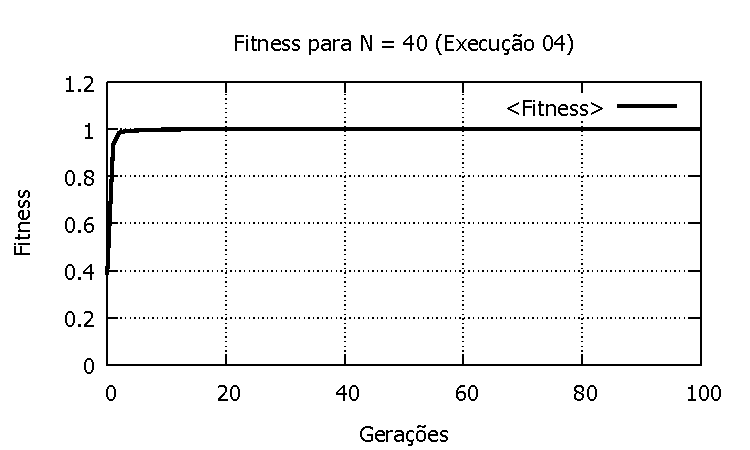
\includegraphics[width=.40\textwidth]{figs/resultados/N40_04_fitness.pdf} &
    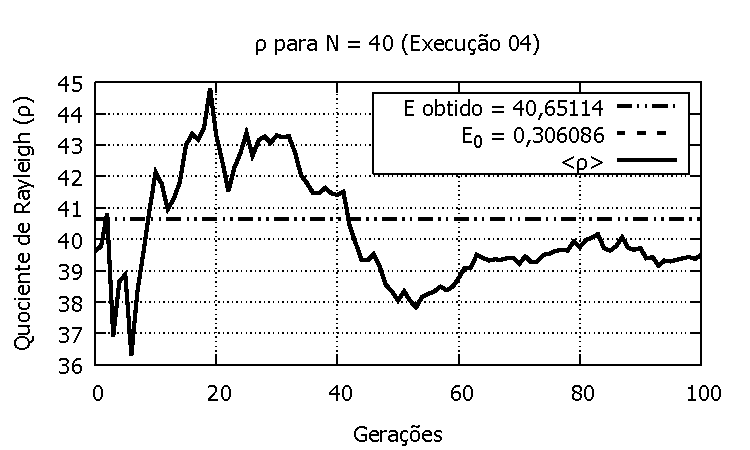
\includegraphics[width=.40\textwidth]{figs/resultados/N40_04_rho.pdf}   \\
		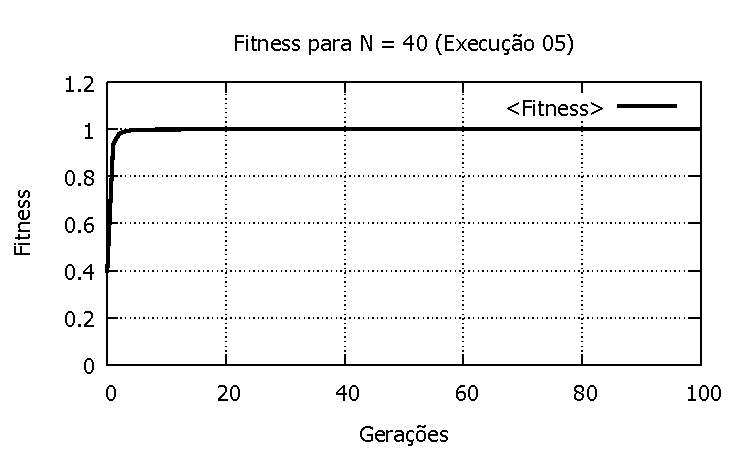
\includegraphics[width=.40\textwidth]{figs/resultados/N40_05_fitness.pdf} &
    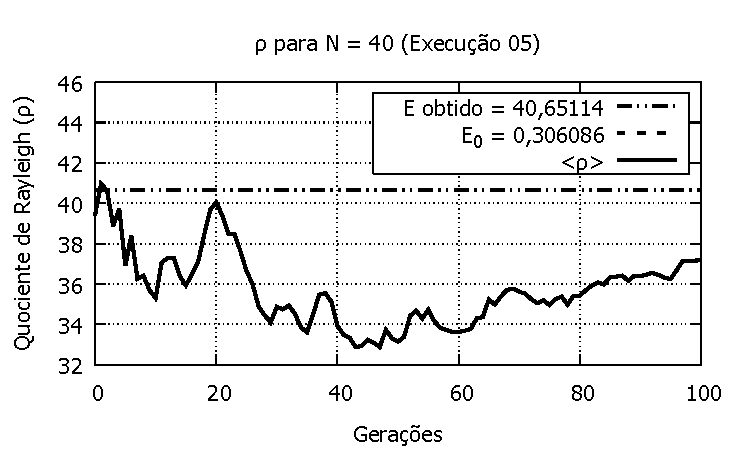
\includegraphics[width=.40\textwidth]{figs/resultados/N40_05_rho.pdf}
    %\multicolumn{2}{c}{\includegraphics[width=.23\textwidth]{example-image-a}}
  \end{tabular}
  \caption{Execuções N = 40.}
	\label{fig:execucoes_N40}
\end{figure}

\newpage
\begin{landscape}
\begin{center}
\begin{table}[htbp]
\caption{Execuções para matrizes de Coope$-$Sabo.}
\label{tab:execucoes10a40}
% Table generated by Excel2LaTeX from sheet 'Plan1 (2)'
\begin{tabular}{cccccccccc}
\hline \hline
   \textbf{N} & \textbf{Execução} & \textbf{Semente} & \textbf{$\lambda$} & \textbf{<\textit{Fitness}>} & \textbf{<$\rho$>} & \textbf{$\sigma$} & \textbf{\# autovalor} & \textbf{Autovalor} & \textbf{Erro relativo} \\
\hline \hline
        10 &          0 & 1445738835 &   0,128788 &   1,000000 &   2,461122 &   0,000023 &          1 &   2,461056 &    0,003\% \\
\hline
        10 &          1 & 1445780626 &   0,128788 &   1,000000 &   6,572898 &   0,000013 &          3 &   6,572897 &  0,00001\% \\
\hline
        10 &          2 & 1445780762 &   0,128788 &   1,000000 &   6,572883 &   0,000015 &          3 &   6,572897 &  -0,0002\% \\
\hline
        10 &          3 & 1445780907 &   0,128788 &   1,000000 &   6,572910 &   0,000016 &          3 &   6,572897 &   0,0002\% \\
\hline
        10 &          4 & 1445781049 &   0,128788 &   1,000000 &  12,765701 &   0,000016 &          6 &  12,765740 &  -0,0003\% \\
\hline
        10 &          5 & 1445781195 &   0,128788 &   1,000000 &   4,518952 &   0,000012 &          2 &   4,518931 &   0,0005\% \\
\hline
        20 &          1 & 1445795292 &   0,026665 &   1,000000 &   8,498192 &   0,000052 &          4 &   8,497626 &    0,007\% \\
\hline
        20 &          2 & 1445795501 &   0,026665 &   1,000000 &  12,551830 &   0,000018 &          6 &  12,551780 &   0,0004\% \\
\hline
        20 &          3 & 1445795718 &   0,026665 &   1,000000 &  12,551878 &   0,000020 &          6 &  12,551780 &   0,0008\% \\
\hline
        20 &          4 & 1445795953 &   0,026665 &   1,000000 &  14,578527 &   0,000035 &          7 &  14,578450 &   0,0005\% \\
\hline
        20 &          5 & 1445796166 &   0,026665 &   1,000000 &  18,634220 &   0,000062 &          9 &  18,633850 &    0,002\% \\
\hline
        30 &          1 & 1445796378 &   0,011171 &   1,000000 &  26,616790 &   0,000065 &         13 &  26,616670 &   0,0005\% \\
\hline
        30 &          2 & 1445796746 &   0,011171 &   1,000000 &  26,616595 &   0,000029 &         13 &  26,616670 &  -0,0003\% \\
\hline
        30 &          3 & 1445797109 &   0,011171 &   1,000000 &  22,580060 &   0,000051 &         11 &  22,580300 &   -0,001\% \\
\hline
        30 &          4 & 1445797473 &   0,011171 &   1,000000 &  40,772447 &   0,000071 &         20 &  40,772850 &   -0,001\% \\
\hline
        30 &          5 & 1445797882 &   0,011171 &   1,000000 &  30,655283 &   0,000022 &         15 &  30,655270 &  0,00004\% \\
\hline
        40 &          1 & 1445798248 &   0,006105 &   1,000000 &  26,554758 &   0,000040 &         13 &  26,554690 &   0,0003\% \\
\hline
        40 &          2 & 1445798838 &   0,006105 &   1,000000 &  54,773734 &   0,000078 &         27 &  54,773690 &  0,00008\% \\
\hline
        40 &          3 & 1445799429 &   0,006105 &   1,000000 &  58,819413 &   0,000087 &         29 &  58,819810 &  -0,0007\% \\
\hline
        40 &          4 & 1445800091 &   0,006105 &   1,000000 &  40,651473 &   0,000077 &         20 &  40,651140 &   0,0008\% \\
\hline
        40 &          5 & 1445800683 &   0,006105 &   1,000000 &  40,650764 &   0,000061 &         20 &  40,651140 &  -0,0009\% \\
\hline \hline
\end{tabular}
\end{table}  
\end{center}
\end{landscape}

\newpage

	
\begin{table}[pt]
	\caption{Autovalores para matrizes de Coope$-$Sabo de ordem 10, 20, 30 e 40.}
	\label{tab:autovalores10a40}
% Table generated by Excel2LaTeX from sheet 'Todos'
\begin{center}
\begin{tabular}{r|r|r|r|r}
	\hline \hline
		 \textbf{\#} &   \textbf{10} &   \textbf{20} &   \textbf{30} &   \textbf{40} \\
	\hline \hline
					 0 &   0,386075 &   0,341237 &   0,319737 &   0,306086 \\
	\hline
					 1 &   2,461056 &   2,397247 &    2,36844 &   2,350583 \\
	\hline
					 2 &   4,518931 &   4,436173 &   4,401134 &   4,379909 \\
	\hline
					 3 &   6,572897 &   6,468521 &   6,427419 &     6,4031 \\
	\hline
					 4 &   8,628524 &   8,497626 &   8,450274 &    8,42294 \\
	\hline
					 5 &   10,69057 &   10,52507 &   10,47105 &   10,44068 \\
	\hline
					 6 &   12,76574 &   12,55178 &    12,4905 &     12,457 \\
	\hline
					 7 &   14,86753 &   14,57845 &   14,50908 &   14,47232 \\
	\hline
					 8 &   17,03654 &   16,60562 &   16,52713 &   16,48692 \\
	\hline
					9 &   22,07215 &   18,63385 &   18,54488 &     18,501 \\
	\hline
					10 &            &    20,6637 &   20,56255 &    20,5147 \\
	\hline
					11 &            &   22,69588 &    22,5803 &   22,52816 \\
	\hline
					12 &            &   24,73127 &   24,59828 &   24,54146 \\
	\hline
					13 &            &   26,77114 &   26,61667 &   26,55469 \\
	\hline
					14 &            &   28,81733 &    28,6356 &   28,56792 \\
	\hline
					15 &            &   30,87288 &   30,65527 &   30,58122 \\
	\hline
					16 &            &   32,94325 &   32,67586 &   32,59466 \\
	\hline
					17 &            &   35,04014 &    34,6976 &   34,60831 \\
	\hline
					18 &            &   37,19805 &   36,72077 &   36,62223 \\
	\hline
					19 &            &    45,2308 &   38,74571 &   38,63648 \\
	\hline
					20 &            &            &   40,77285 &   40,65114 \\
	\hline
					21 &            &            &   42,80277 &    42,6663 \\
	\hline
					22 &            &            &   44,83625 &   44,68204 \\
	\hline
					23 &            &            &   46,87444 &   46,69846 \\
	\hline
					24 &            &            &   48,91902 &   48,71568 \\
	\hline
					25 &            &            &   50,97274 &   50,73385 \\
	\hline
					26 &            &            &   53,04052 &   52,75311 \\
	\hline
					27 &            &            &   55,13271 &   54,77369 \\
	\hline
					28 &            &            &   57,27946 &   56,79581 \\
	\hline
					29 &            &            &   68,37101 &   58,81981 \\
	\hline
					30 &            &            &            &   60,84608 \\
	\hline
					31 &            &            &            &   62,87517 \\
	\hline
					32 &            &            &            &   64,90781 \\
	\hline
					33 &            &            &            &   66,94504 \\
	\hline
					34 &            &            &            &   68,98845 \\
	\hline
					35 &            &            &            &   71,04053 \\
	\hline
					36 &            &            &            &   73,10578 \\
	\hline
					37 &            &            &            &   75,19353 \\
	\hline
					38 &            &            &            &   77,33102 \\
	\hline
					39 &            &            &            &   91,50634 \\
	\hline \hline
	\end{tabular}
	\end{center}  
\end{table}
	
	
	Explicar retomando os fatos sobre cociente de Rayleigh apresentados no (futuro) capítulo de álgebra linear.
	
	Apesar de não chegar ao mínimo, pode ser utilizado de maneira exploratória. Relembrar as dez execuções anteriores e verificar que houve diferentes autovalores encontrados.
	
	Problema: lentidão. Ponte para ...
	
	\section{$f_i = e^{[-\lambda \nabla \rho]}$ é mais rápido do que $f_i = e^{[-\lambda (\nabla \rho)^2]}$}
	
	Como um dos critérios de parada utiliza $\nabla \rho$ (sem quadrado), testamos essa forma no fitness.
	
	Várias execuções.
	
	Gráfico comparando o comportamento (um termina mais rápido)
	
	Tabela com os detalhes explícitos do do ganho.
	
	Ponte pra falar sobre o outro fitness que encontra o mínimo.
	
	\section{$f_i = e^{-\lambda(\rho_i - \rho_0)^2}$ leva ao autovalor mínimo ($E_0$), mas devemos saber aproximadamente onde ele está}
	
	Justificar esse outro fitness com o artigo de 2006.
	
	Discutir a introdução do novo parâmetro $\rho_0$.
	
	Com $\rho = 0$, realizar exatamente as mesmas execuções da seção anterior.
	
	Realizar dez execuções com precisão boa para N = 10 e N = 100;
	
	Verificar que foi possível chegar no mínimo autovalor.
	
	Exemplos de execução:
	
	
	\begin{enumerate}
		\item \textbf{O que acontece quando $\rho_0$ está um pouco acima de $E_0$?}
		
				Para com $<\rho> \approx \rho_0$
				
				Não encontra o menor autovalor ($E_0$).
				
				Porém, verifica-se que o $<\nabla \rho> \approx 0$.
				
				Então, estamos próximos ao menor autovalor.

				
		\item \textbf{O que acontece quando $\rho_0$ está um pouco abaixo de $\lambda_0$}
						
				Encontra uma aproximação para o autovalor mínimo ($\lambda_0$).
				
				$<fitness>$ é próximo a 1 pois $<\rho>$ é próximo de $\rho_0$.
				
				$<\nabla \rho> \approx 0$.
				
						
		\item \textbf{O que acontece quando $\rho_0$ está muito acima de $E_0$?}
		
					Acredito que não encontrará uma aproximação para $E_0$, pois a região de busca está muito distante. (verificar)
					
				Para com $<\rho> \approx \rho_0$
				
				Verifica-se que o $\nabla \rho >> 0$. Portanto, estamos distantes do menor autovalor.
						
		\item \textbf{O que acontece quando $\rho_0$ está muito abaixo de $E_0$?}
				
				Acredito que não encontrará uma aproximação para $E_0$, pois a região de busca está muito distante.
				
				Para com $<\rho> \approx \rho_0$
				
				Verifica-se que o $\nabla \rho >> 0$. Portanto, estamos distantes do menor autovalor.
		
	\end{enumerate}
	
	Citar brevemente a relação entre a dificuldade (parece uma inércia) de melhorar a precisão dos resultados no final, dizer que isso está relacionado com o formato da função \textit{fitness}.
	
	Ponte para a discussão do \textit{fitness}
	
\section{$f_i = e^{-\lambda(\rho_i - \rho_0)^2}$ próximo de $\rho$ é intrinsicamente impreciso}
	
	Como $\lambda$ e $\rho_0$ são constantes por definição, $f_i$ é uma função apenas de $\rho$.
	
	Função simétrica em torno de $\rho_0$.
	
	Gráfico com diferentes $\rho_0$'s para o domínio $\rho = [-200,200]$. 
	
	Para uma dada função $fitness$, em torno de zero, por exemplo, dar um \textit{zoom} no pico.
	
	\begin{figure}[htbp]
		\centering
			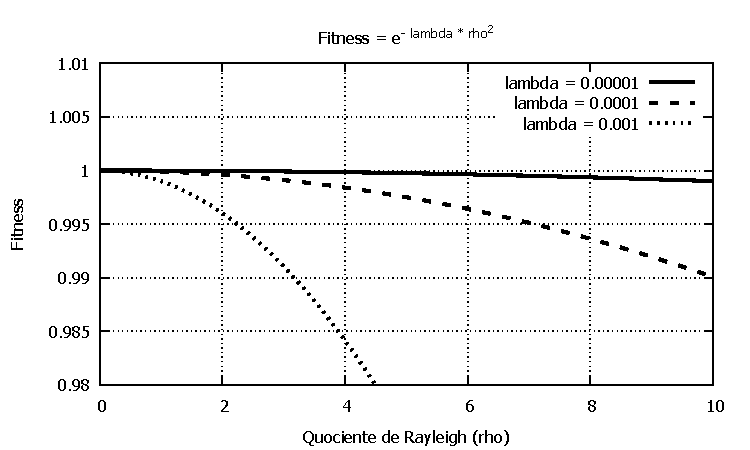
\includegraphics{figs/varios-fit-mono-zoom.pdf}
		\caption{Zoom próximo do pico}
		\label{fig:varios-fit-mono-zoom}
	\end{figure}
	
	
	Gráficos com $\rho = [-5,5]$ e $\rho = [-0.1,+0.1]$.
	
	Verificar que no último gráfico o SciLab já apresenta dificuldades para diferenciar os pontos de $f$.
	
	Gráfico da variação do fitness como função da variação do $\rho$ (a derivada).
	
	A derivada é 
	
	$$
		\frac{df}{d\rho} = -2\lambda(\rho - \rho0)e^{-\lambda(\rho - \rho0)^2}
	$$
	
	Com $\rho = [-200,200]$, gráfico da derivada.
	
	Gráfico comparando $f$ com $df/d\rho$. Verificar visualmente que $df/d\rho$ é muito pequeno, próximo de zero. 
	
	Tabela com os valores mostrando que, próximo à $\rho_0$, uma mudança de $\Delta\rho = 0.1$ leva a uma variação de $\Delta f <= 0.000001$.
	
	Para o algoritmo genético isso é ruim. Cada rho está associado a um indivíduo e o fitness deve diferenciar cada um, de modo que a maior nota é dada ao indivíduo mais próximo da solução.
	
	Veja que para $\rho = [-0.3,+0.3]$ o fitness é igual a 1. Nessa região a o fitness falha na diferenciação dos indivíduos.
	
	Para fitness muito pequeno há o mesmo problema. Com isso, pode-se definir uma região do fitness onde a função é apropriada para o uso dos algoritmos genéticos. Figura \ref{fig:fitness_boaRegiao}.
	
	Para Futuro, continuação do trabalho: há alguma maneira de lidar com os parâmetros de $f$ de modo a ficarmos sempre na região boa?
	
	Região boa: entre as duas linhas, quase linear.
		
	\begin{figure}[htbp]
		\centering
			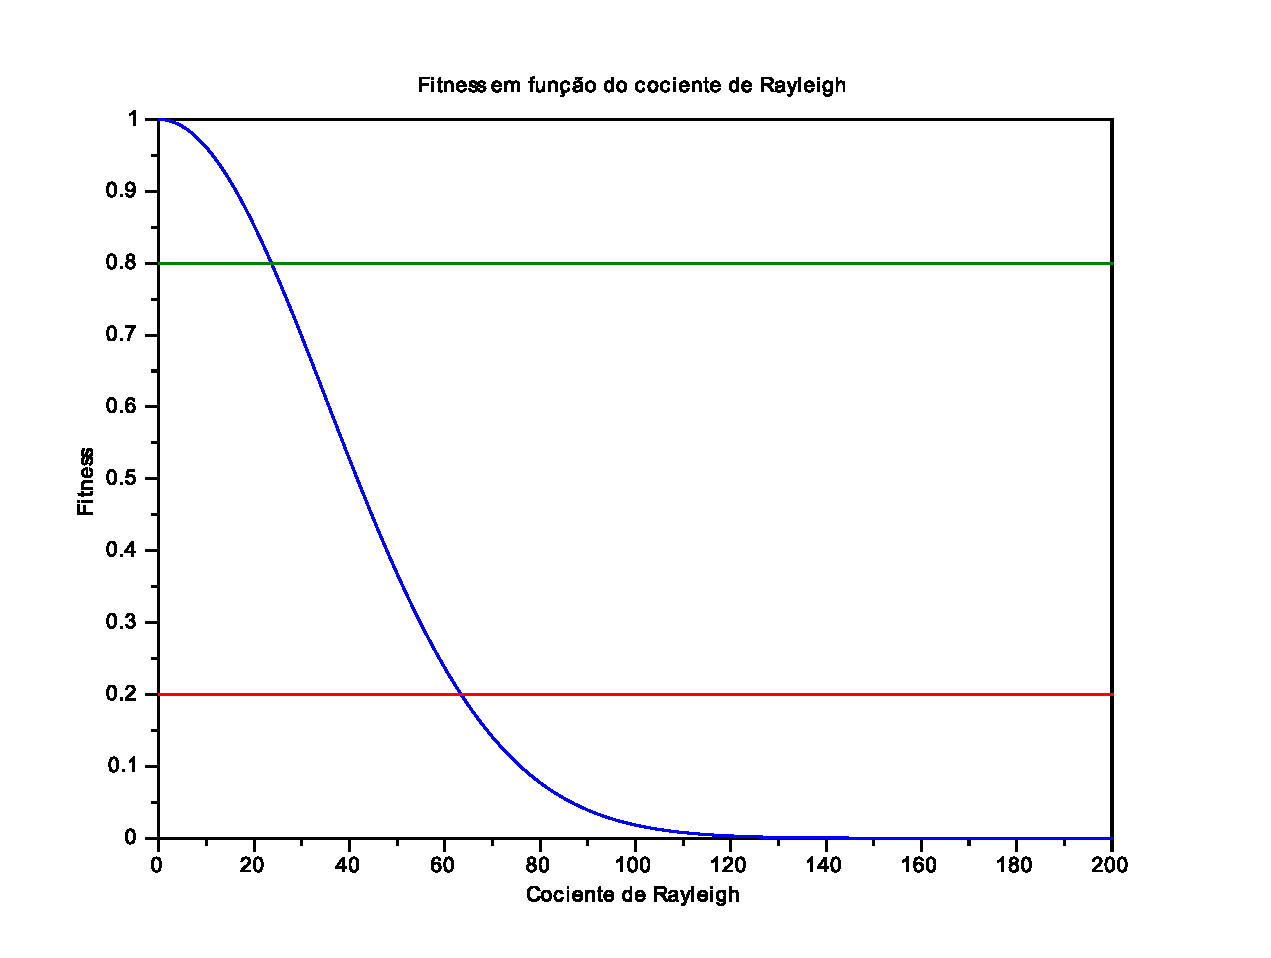
\includegraphics[width=0.90\textwidth]{figs/resultados/fitness_boaRegiao.pdf}
		\caption{Boa região para o fitness (entre as duas linhas)}
		\label{fig:fitness_boaRegiao}
	\end{figure}
	
	Há um limite de precisão intrínseco com o uso desse fitness.
	
	Por isso a dificuldade em melhorar a precisão.
	
	% Table generated by Excel2LaTeX from sheet 'Plan2'
\begin{tabular}{rr}

       \textit{rho} &          \textit{f} \\

      -0,1 &   0,999996 \\

     -0,09 &   0,999997 \\

     -0,08 &   0,999997 \\

     -0,07 &   0,999998 \\

     -0,06 &   0,999999 \\

     -0,05 &   0,999999 \\

     -0,04 &   0,999999 \\

     -0,03 &          1 \\

     -0,02 &          1 \\

     -0,01 &          1 \\

         0 &          1 \\

      0,01 &          1 \\

      0,02 &          1 \\

      0,03 &          1 \\

      0,04 &   0,999999 \\

      0,05 &   0,999999 \\

      0,06 &   0,999999 \\

      0,07 &   0,999998 \\

      0,08 &   0,999997 \\

      0,09 &   0,999997 \\

       0,1 &   0,999996 \\

\end{tabular}  

		
		O parâmetro $\lambda$ também influencia fortemente o fitness e o algoritmo genético.
		
		Ponte para a discussão do $\lambda$.
		
	\section{Por que o $\lambda$ deve ser escolhido cuidadosamente?}
	
	Execuções para N=10 com diferentes $\lambda$'s. Com os gráficos, explicar o que o artigo de 2004 quis dizer com \textit{fitness overflow/underflow}.
	
	Gráficos com rho entre 0 e 250 (exemplo pra N=10), mas com cortes em diferentes rhos.
	
	\begin{figure}[pt]
	\centering
		\includegraphics{figs/varios-fits-color.pdf}
	\caption{Fitness em função do lambda $-$ colorido}
	\label{fig:varios-fits-color}
\end{figure}

\begin{figure}[pb]
	\centering
		\includegraphics{figs/varios-fits-mono.pdf}
	\caption{Fitness em função do lambda}
	\label{fig:varios-fits-mono}
\end{figure}

	Explicar que uma boa escolha do $\lambda$ deve cobrir todos os autovalores. Citar as execuções anteriores (boas e ruins em função de cada $\lambda$).
	
	Gráfico com $\lambda$ fazendo o fitness cortar em um $\rho$ muito baixo. Discutir puxando as execuções anteriores.
	
	Outro gráfico, mas com $\lambda$ fazendo o fitness cortar em um $\rho$ muito alto. Discutir puxando as execuções anteriores.
	
	Gráfico com uma boa escolha de $\lambda$. Discutir puxando as execuções anteriores.
	
	Após estimativa, refinar a obtenção do $\lambda$. Alterar o $lambda$ (valores em torno da estimativa), executar o programa para verificar se o fitness médio da primeira população é baixo. (se a população inicial tem fitness muito grande, há convergência prematura).
	
	Tabela com alguns $lambdas$ encontrados dessa maneira (estimativa e refinamento).
	
	Infelizmente, para cada matriz, um $\lambda$ diferente.
	
	Ponte pra equação empírica do $\lambda$.
	
	\section{Equação empírica para o $\lambda$}
	
	Delineamento da equação como feito na reunião de 29/09.
	
	Isolar $\lambda$ a partir da $f=e^{-\lambda*(\rho - \rho_0)^2}$
	
	Fazer $f = 0.00001 \approx 0$.
	
	Substituir $(\rho - \rho_0)^2$ por $E_{central} - E_{mínimo}$. Justificar.
	
	Regressão linear para $E_{central} - E_{mínimo}$ com função apenas da ordem da matriz (N).
	
	Inserir a Equação obtida na regressão na equação de $\lambda$.
	
	Fator $0.65$: obtido empiricamente de modo que o $\lambda$ seja semelhante aos encontrados pelo processo de estimativa e refinamento.
	
	Exemplo de execução com $\lambda$ automático.
	
	Explicitar que essa equação é válida apenas para matrizes de Coope$-$Sabo. Apesar disso, foi importante para o estudo pois permitiu automação completa.
		
	\section{A mistura de $(\rho - \rho_0)^2$ com $\nabla\rho$ não leva a melhores resultados}
	
	Como em seção anterior verificamos que $f_i = e^{[-\lambda \nabla \rho]}$ é mais rápido do que $f_i = e^{[-\lambda (\nabla \rho)]}$, e que o $\nabla\rho$ está diretamente associado aos autovalores, pensei na seguinte hipótese: inserir $\nabla \rho$ ao fitness com $(\rho - \rho_0)^2$ traria resultados mais rápidos.
	
	Justificativas para a hipótese: 
	
	\begin{enumerate}
		\item Inserir $\nabla \rho$ no fitness puniria os $\rho$'s que, apesar de próximos de $\rho_0$, não fossem autovalor. Em outras palavras, o termo $\rho - \rho_0 \approx 0$, mas $\nabla \rho >> 0$ e, portanto, o fitness ficaria pequeno.
		
		\item Como o fitness, a princípio, estaria diferenciamento melhor os bons indivíduos, o algoritmo teria uma taxa de convergência maior.
		
	\end{enumerate}
	
		Executar $10$ para o primeiro fitness, e, utilizando as mesmas dez sementes, executar outros $10$ testes com ou outro fitness.
		
		Comparação dos resultados: gráficos do comportamento do fitness e tabela comparando a velocidade de convergência (em que geração o critério de parada foi atingido), tempo de execução e erro relativo ao menor autovalor ``exato'' (obtido no SciLab).
	
	\section{Resultados preliminares na GPU}
	
		\subsection{ONEMAX na GPU}
	
				ERAD: artigo $+$ poster
				
		\subsection{Método paralelizado (versão atual, com ganho de $1,4$}
		
				Falar um pouco.
		
				